% Template for the Project 3 research article. Do not edit numbers here: tokens like 290 are
% filled from report/stats.json and report/analysis.json by code/08_paper.py, which writes paper/main.tex.
\documentclass[11pt]{article}
\usepackage[margin=1in]{geometry}
\usepackage{setspace}
\onehalfspacing
\usepackage[T1]{fontenc}
\usepackage{lmodern}
\usepackage{graphicx}
\usepackage{booktabs}
\usepackage{caption}
\captionsetup{font=small,labelfont=bf,justification=raggedright,singlelinecheck=false}
\usepackage[authoryear,round]{natbib}
\usepackage{xcolor}
\definecolor{linkblue}{RGB}{28,92,171}
\usepackage[colorlinks=true,linkcolor=black,citecolor=linkblue,urlcolor=linkblue]{hyperref}
\hypersetup{pdftitle={Where Safety Plans Have Not Reached: Safe Streets and Roads for All Action Plan Coverage and Rural Traffic Deaths in U.S. Counties, Fiscal Years 2022--2026},pdfauthor={Emmanuel Oti Nani; Sedinam Annie Barney},pdfkeywords={road safety; Safe Streets and Roads for All; safety action plans; rural roads; traffic fatalities}}
\usepackage{orcidlink}
\usepackage{lineno}
\usepackage{float}


\title{\textbf{Where Safety Plans Have Not Reached: Safe Streets and Roads for All Action Plan Coverage and Rural Traffic Deaths in U.S.\ Counties, Fiscal Years 2022--2026}}
\author{Emmanuel Oti Nani\,\orcidlink{0009-0009-4175-8962}\\[2pt]\small Independent Researcher, Springfield, Missouri, USA\\\small \href{mailto:en289s@missouristate.edu}{en289s@missouristate.edu} (corresponding author)\\[10pt]Sedinam Annie Barney\,\orcidlink{0009-0001-1017-6451}\\[2pt]\small Independent Researcher}
\date{}

\begin{document}
\maketitle
\linenumbers

\begin{abstract}
\noindent The Safe Streets and Roads for All (SS4A) program was established under the Infrastructure Investment and Jobs Act to support road safety planning and projects by local, regional, and Tribal governments during fiscal years 2022 through 2026. A comprehensive safety action plan is a prerequisite for an SS4A implementation grant, making the reach of these plans an important question. This study brings together all 2{,}659 SS4A awards (\$4.93 billion), checks them against the U.S.\ Department of Transportation's official lists, maps their geographic coverage to counties using 2020 Census block-group population centers, and compares that coverage with county traffic deaths from 2020 to 2024. Although about 71\% of U.S.\ residents live within an SS4A-funded action plan area, plans covered 62\% of urban counties and 37\% of rural counties, where the death rate is twice as high. Across the five funding rounds, the urban--rural coverage gap increased from 20 to 26 percentage points. Among the 448 rural counties with the highest death rates, 290 (65\%) still lack a funded plan covering most residents. These counties accounted for 4.1\% of national traffic deaths but received only 0.7\% of SS4A dollars. The regression results indicate that population and urbanization, rather than fatality burden, poverty, or income, were associated with coverage. State location accounted for about a third of the variation among rural counties. Early plans were also followed by construction funding more often in urban counties (27\% of early-covered counties) than in rural counties (7\%). In those 290 counties, 73\% of deaths occurred on state-owned roads. Gaps tend to cluster geographically, while states with established local road safety programs had lower rural SS4A coverage, consistent with the existence of plans supported through other sources. DOT's lists of eligible but unfunded applications show that only 7 gap counties had an application turned down, while rural and urban applicants were funded at similar rates, so the gaps arose mainly because counties did not apply. Defining high fatality by deaths per mile traveled leaves the pattern unchanged. Taken together, the results show that this competitive, application-driven program reached most Americans but was least likely to cover the rural counties with the highest traffic death rates.\\[6pt]
\noindent\textbf{Keywords:} road safety; Safe Streets and Roads for All; safety action plans; rural roads; traffic fatalities; regional planning; grant distribution; spatial analysis
\end{abstract}

\section{Introduction}

Rural communities continue to experience considerably higher traffic death rates than urban areas. According to the National Highway Traffic Safety Administration, rural areas accounted for 41\% of traffic deaths in 2024, although only about 21\% of Americans live there \citep{nhtsa2026}. A similar difference appears in the county-level data used here. Between 2020 and 2024, counties in which most residents lived outside Census urban areas averaged 21.9 traffic deaths per 100{,}000 residents per year, compared with 10.7 in urban counties \citep{nani2026panel}. Earlier research has linked this rural disadvantage to higher travel speeds, longer emergency response times, lower seat belt use, and road designs that provide less protection when drivers make mistakes \citep{zwerling2005,peekasa2004,beck2017,henningsmith2018}.

Congress established the Safe Streets and Roads for All (SS4A) program through the Infrastructure Investment and Jobs Act (IIJA) in 2021, appropriating \$5 billion for fiscal years 2022 through 2026 \citep{iija2021,dotss4a}. The program provides direct federal support to local governments, metropolitan planning organizations (MPOs), regional councils, and Tribal governments for road safety plans and projects. It follows the Safe System Approach set out in the National Roadway Safety Strategy \citep{itf2016,nrss2022}. At the center of SS4A is the comprehensive safety action plan, which uses data to identify locations with deaths and serious injuries and sets out measures to prevent them. At least 40\% of annual funding must support the development of such plans \citep{fhwass4a}. Communities must also have an eligible plan before receiving an implementation grant for projects \citep{dotss4a}. SS4A plan coverage therefore shapes which places can take the next step toward construction funding under the program.

Access to SS4A funding depends on a competitive application process. Applicants must establish eligibility, prepare proposals, and provide a 20\% local match. These requirements may be easier to meet in communities with dedicated planning staff and grant-writing resources. Research using a national measure of rural government capacity finds that greater capacity predicts success in competitive federal resilience grants \citep{smith2025}. A journalistic analysis of SS4A's early rounds also found that most funding went to counties with lower fatality rates \citep{fast2024}. Many small towns and rural counties do not have their own planning staff and instead depend on regional councils, regional planning organizations, or state technical assistance to prepare safety plans \citep{fhwa2012,fhwa2014}. Some states have also operated programs for many years to help local agencies plan safety improvements on locally owned roads \citep{anderson2010}.

Despite growing attention to SS4A, no published assessment known to the authors has mapped the places reached by its funded action plans across all five rounds. DOT reports each round separately, and the files vary in their fields and labels. Moreover, an award may serve only part of one county or extend across several counties, so counting awards by county does not establish how many residents are actually within a funded plan area. To address this problem, the study develops an award-level record linked to the places each award covers. It examines the proportion of urban and rural populations within funded action plan areas and how coverage changed across rounds, with particular attention to rural counties experiencing the highest death rates. It then considers the county characteristics associated with coverage, whether early plans were followed by construction funding in rural and urban communities, and how program dollars compare with traffic deaths. Finally, it examines road ownership in uncovered counties, the geographic concentration of coverage gaps, and differences among states.

Section~\ref{sec:background} provides the program background, followed by the award data and reconciliation process in Section~\ref{sec:data}. Section~\ref{sec:methods} explains how coverage was measured and analyzed. The results appear in Section~\ref{sec:results}, with their implications and limitations discussed in Section~\ref{sec:discussion}. Section~\ref{sec:conclusion} concludes.

\section{Program background}\label{sec:background}

SS4A provides two grant categories with different purposes. Planning and Demonstration Grants, known as Action Plan Grants in the first round, support the preparation or revision of comprehensive safety action plans. They can also fund activities such as road safety audits, data analysis, and temporary demonstrations of safety measures. Implementation Grants, often worth millions of dollars, support the infrastructure, behavioral, and operational projects identified in those plans \citep{dotss4a}. Cities, towns, counties, special districts, and other political subdivisions of states are eligible, as are MPOs and federally recognized Tribal governments. Applicants may also work together, allowing a regional council, for example, to prepare one safety plan for several smaller jurisdictions.

The law reserves no less than 40\% of each year's funding for action plans \citep{fhwass4a}. For grant scoring, however, SS4A uses a broader rural definition than the Census Bureau: it includes jurisdictions outside urban areas as well as those within urban areas of fewer than 200{,}000 people. DOT reports that about half of the awards in each round went to communities classified as rural under that definition. This is an award count rather than a measure of the population or fatalities reached. The distinction is important when interpreting the differences in rural and urban plan coverage reported in this study.

\section{Data}\label{sec:data}

\subsection{SS4A awards}

The study draws on two DOT sources for each funding round: the official award map layers hosted on ArcGIS Online and the corresponding spreadsheet award lists \citep{dotlayers,dotlists}. The layers identify recipients, states, grant programs, activities, federal funding amounts, and the boundaries of the areas served. The final map layer for each fiscal year (FY) from 2022 through 2026 was retrieved in November 2026. Contact details and internal DOT notes were excluded from the dataset.

The map records were checked against DOT's official award lists for all five years. Awards from FY2022 were matched individually using the Unique Entity Identifier; those from FY2023 through FY2026 were matched using state, grant program, federal funding, and recipient name. After reconciliation, all 2{,}659 awards matched the official lists on recipient, state, program, funding, and DOT's rural or urban designation. Several corrections were necessary. Two FY2022 action plan awards appeared in the list but in none of the year's map layers, so they were included without mapped boundaries. One state code was corrected, and 52 FY2026 implementation awards marked rural in the map layer were changed to urban to match the list. In addition, 3 award areas had been drawn around similarly named towns or counties in other states. These were replaced with the 2020 Census boundaries of the recipients identified in the official lists. Table~\ref{tab:fy} reports the reconciled awards by fiscal year.

\begin{table}[H]
\centering
\caption{SS4A awards by fiscal year after reconciliation with DOT's award lists. Action plan awards fund developing or updating a comprehensive safety action plan; regional bodies are regional councils and MPOs.}
\label{tab:fy}
\small
\begin{tabular}{lrrrrr}
\toprule
Fiscal year & Awards & Federal funding (\$ million) & Implementation & Action plan & To regional bodies \\
\midrule
FY2022 & 511 & 802 & 37 & 450 & 114 \\
FY2023 & 620 & 896 & 48 & 455 & 51 \\
FY2024 & 710 & 1{,}241 & 70 & 455 & 35 \\
FY2025 & 521 & 982 & 67 & 283 & 26 \\
FY2026 & 297 & 1{,}013 & 100 & 97 & 7 \\
\midrule
Total & 2{,}659 & 4{,}935 & 322 & 1{,}740 & 233 \\
\bottomrule
\end{tabular}
\end{table}

\subsection{Population, boundaries, and county characteristics}

Geographic boundaries for counties, Census places, and New England county subdivisions were taken from the Census Bureau's 2020 cartographic boundary files \citep{censuscb}. Residents were located using the 2020 population centers of 242{,}335 block groups, which provide both the 2020 population count and the average residential location for each group \citep{censuscenpop}. County-level poverty rates and median household incomes for 2023 were obtained from the Census Bureau's Small Area Income and Poverty Estimates \citep{saipe2023}.

\subsection{Traffic deaths}

Traffic deaths were obtained from the U.S.\ Rural Road Fatality County Panel (version 1.0.0), an open county-by-year dataset based on Fatality Analysis Reporting System (FARS) records for 2015 to 2024 and aligned to 2020 county boundaries \citep{nani2026panel}. This analysis uses deaths recorded from 2020 to 2024, annual Census population estimates, and the proportion of each county's 2020 residents living outside 2020 Census urban areas \citep{census2022}. It also uses the panel's breakdown of deaths by road owner and functional class. Census urban-area boundaries are held constant throughout the panel; a companion study evaluates that choice \citep{nani2026valid}.

\subsection{Unfunded applications and travel}

DOT has published lists of eligible applications that did not receive funding for fiscal years 2022, 2023, and 2024 \citep{usdot2025oa}. The FY2022 list covers implementation applications only, the FY2023 and FY2024 lists cover both grant types, and no lists have been published for FY2025 or FY2026. Together the lists contain 630 applications, each recorded with the lead applicant's name, state, grant type, and DOT's rural or urban designation. Vehicle-miles traveled in 2024 were taken from the Highway Performance Monitoring System \citep{fhwa2024hpms} and summed by county as average annual daily traffic multiplied by section length. This measure, about 2.9 trillion vehicle-miles nationally, covers road sections that carry traffic counts, mostly arterials and collectors, and omits most travel on local roads.

\section{Methods}\label{sec:methods}

\subsection{Coding of awards}

Awards were classified according to their purpose: developing or updating a comprehensive safety action plan, supporting supplemental planning or demonstration activities, or implementing projects. Because an award may support several activities, these categories are not mutually exclusive. Recipients were identified as cities, counties, Tribes, MPOs, regional councils, or other organizations. DOT's applicant categories were used where possible, while recipient names helped distinguish MPOs from regional councils, including councils of governments, regional planning commissions, and development districts, that appeared under broader DOT categories. The data repository documents 17 manual corrections and the reasons for them. MPOs and regional councils were also grouped together as regional bodies because many MPOs operate within regional councils.

\subsection{Coverage measures}

An award area was considered to include a block group if the group's 2020 population center fell within the mapped boundary. For each county, coverage was measured as the proportion of 2020 residents living in block groups included in at least one funded action plan area; overlapping awards were counted only once. Counties with coverage of at least one half were classified as covered, those with positive coverage below one half as partly covered, and those with no coverage as not covered. The main measure includes action plan awards from FY2022 through FY2026. Two alternative measures account for limitations in the DOT maps. In 55 cases, the mapped action plan area contained more than twice the population DOT attributed to the recipient's jurisdiction, sometimes because a plan intended for unincorporated areas was mapped across an entire county. The conservative measure excludes those awards. A second measure omits the final funding round, whose plans are the least likely to have been completed.

Rural status was defined using the 2020 Census urban-area boundaries. A county was considered rural if at least half of its 2020 population lived outside those areas, yielding 2{,}010 rural counties among the 3{,}143 counties in the 50 states and the District of Columbia. Traffic fatality burden was calculated as deaths from 2020 to 2024 per 100{,}000 residents per year. To identify high-fatality rural counties, the analysis retained rural counties with at least 5 deaths over the period and classified those in the top quarter of the resulting death-rate distribution as high fatality. The cutoff was 33.1 deaths per 100{,}000 residents per year, identifying 448 counties. High-fatality rural counties without majority plan coverage were designated gap counties. For each, the analysis also identified regional bodies with action plans extending into a bordering county as potential partners.

\subsection{Analyses}

Changes in coverage were tracked by recalculating each county's covered population after every fiscal year of awards. The transition from planning to construction funding was assessed at both the county and recipient levels. For counties covered by action plans in the first two rounds (FY2022 and FY2023), the analysis checked whether any residents subsequently fell within implementation award areas from FY2023 through FY2026. Separately, recipients awarded an action plan grant in FY2022 or FY2023 were matched to later implementation awards made to the same recipient in the same state.

To compare the geographic distribution of funding with traffic deaths, each award's federal dollars were assigned to counties according to the proportion of residents served in each county. If an award area contained no block-group population center, the award was assigned to the county in which that area lay. Funding was then totaled by county group, distinguishing planning and demonstration awards from implementation awards, and expressed per resident and per death from 2020 to 2024. For each county group, the analysis also summarized the roads on which deaths occurred by ownership and functional class.

Four models were estimated to assess which county characteristics were associated with plan coverage. The first used logistic regression to model whether a county was covered, with predictors including the logarithm of its 2020 population, the share of residents living in rural areas (per 10 percentage points), the death rate (per 10 deaths per 100{,}000 per year, capped at 200 to reduce the influence of sparsely populated counties), the 2023 poverty rate, and the logarithm of 2023 median household income. Census region indicators were included. A linear probability model with state fixed effects provided a comparison within states, while a fractional logit model examined the share of residents covered rather than a binary coverage indicator \citep{papke1996}. The fourth model repeated the logistic analysis for rural counties alone. All models used state-clustered standard errors and were estimated in statsmodels \citep{seabold2010}; average marginal effects were reported for the logistic specifications. Eight Connecticut counties were omitted because 2023 estimates were published only for the state's new planning regions, as was Kalawao County, Hawaii, for which no estimates were available (3{,}134 counties remain).

Spatial patterns were examined using global Moran's $I$ \citep{moran1950} for both county coverage shares and the gap indicator. The analysis used first-order queen contiguity, row-standardized weights, and 999 permutations. Local Moran statistics \citep{anselin1995} were then used to identify counties with low coverage adjacent to other low-coverage counties. These calculations were carried out in PySAL \citep{rey2007}. To examine differences among states, the analysis measured how much of the variation in rural county coverage could be explained by state alone. It also compared rural coverage in the seven states identified by FHWA as having established local road safety programs (Alabama, Georgia, Illinois, Michigan, Minnesota, New Jersey, and Washington) with coverage elsewhere \citep{anderson2010}.

\subsection{Unfunded applications and travel exposure}

Each unfunded application was placed in the counties holding at least 10\% of the applicant's 2020 population, using Census places, county subdivisions, and counties matched by name within the state. Applicants whose service area could not be read from the name, such as regional councils, tribes, and special districts, were placed by hand from their published service areas; 2 could not be placed. Two comparisons followed. First, each gap county was classified by whether any unfunded application came from within it. Second, funding rates were compared across county groups at the applicant level, limited to rounds in which DOT published both funded and unfunded applicants for the same grant type: implementation grants for FY2022 to FY2024 and planning and demonstration grants for FY2023 and FY2024. Regional applicants were excluded from this comparison because they cannot be assigned to one county; every other applicant was assigned to the county holding most of its population, and differences were tested with chi-square tests.

As a check on the per-resident definition of high-fatality counties, death rates were also expressed per 100 million vehicle-miles traveled, using five times the 2024 travel as exposure for 2020 to 2024, and the top quarter of rural counties with at least five deaths was identified on that basis.

\section{Results}\label{sec:results}

\subsection{The program}

Across the five funding rounds, SS4A made 2{,}659 awards totaling \$4.93 billion. Of these, 1{,}740 supported action plans, including 233 awarded to regional bodies (Table~\ref{tab:fy}). As funding increasingly shifted toward implementation, action plan awards declined from 450 in FY2022 to 97 in FY2026. Awards for action plans led by regional bodies declined in each round as well, from 114 to 7.

\subsection{Coverage by county type}

Funded action plan areas include about 71\% of U.S.\ residents, but their reach differs substantially by county type. They include 75\% of residents in urban counties and 43\% of those in rural counties. Measured by the number of counties rather than residents, 62\% of urban counties were covered, compared with 37\% of other rural counties and 35\% of high-fatality rural counties (Table~\ref{tab:cov} and Figure~\ref{fig:groups}). The urban--rural difference is statistically significant ($\chi^2_1=189.7$, $p<0.001$), whereas coverage in high-fatality and other rural counties does not differ significantly ($\chi^2_1=0.58$, $p=0.44$). Among rural counties with at least 5 deaths, the association between death rate and coverage share is negligible (Spearman $\rho=-0.05$). Excluding potentially overstated award areas or the last funding round changes the reported coverage shares by only a few percentage points.

\begin{table}[H]
\centering
\caption{Counties by funded action plan coverage under three measures. Main: all action plan awards, FY2022--2026. Conservative: excluding awards whose mapped area holds more than twice the population DOT reports. FY2022--2025: excluding the final round. Death rates are per 100{,}000 residents per year, 2020--2024.}
\label{tab:cov}
\small
\begin{tabular}{lrrrrr}
\toprule
 & & & \multicolumn{3}{c}{Counties covered (\%)} \\
\cmidrule(lr){4-6}
County group & Counties & Death rate & Main & Conservative & FY2022--2025 \\
\midrule
Urban & 1{,}133 & 10.7 & 62.5 & 59.2 & 60.8 \\
Other rural & 1{,}562 & 18.7 & 37.4 & 34.4 & 36.3 \\
High-fatality rural & 448 & 45.4 & 35.3 & 33.5 & 32.4 \\
\bottomrule
\end{tabular}
\end{table}

\begin{figure}[H]
\centering
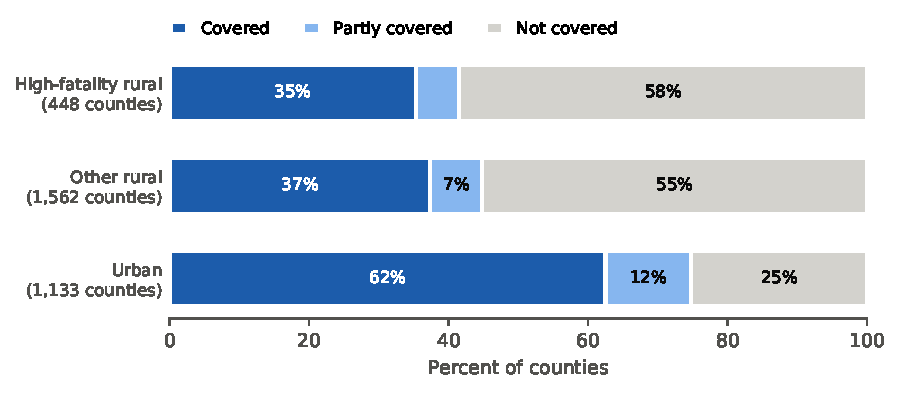
\includegraphics[width=0.72\textwidth]{figures/fig_groups.pdf}
\caption{Share of counties by funded action plan coverage, main measure. Covered: at least half of 2020 residents inside an SS4A action plan area.}
\label{fig:groups}
\end{figure}

\subsection{Coverage across the five rounds}

Although coverage increased with every funding round, it expanded more quickly in urban than in rural counties (Figure~\ref{fig:rounds}). Following the first round, plans covered 34\% of urban counties, 16\% of other rural counties, and just 7\% of high-fatality rural counties. By the fifth round, coverage had reached 62\%, 37\%, and 35\%, respectively. The gap between urban and all rural counties therefore widened from 20 to 26 percentage points. High-fatality rural counties made notable gains in later rounds after starting from the lowest level, but their coverage remained below that of other rural counties through FY2026.

\begin{figure}[H]
\centering
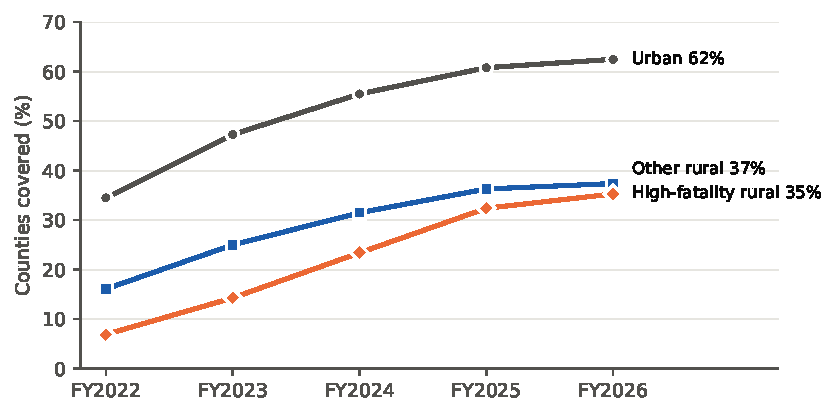
\includegraphics[width=0.72\textwidth]{figures/fig_rounds.pdf}
\caption{Cumulative share of counties covered by SS4A action plans after each funding round, by county group.}
\label{fig:rounds}
\end{figure}

\subsection{Gap counties}

Among the 448 high-fatality rural counties, 290 (65\%) did not have funded action plans covering most residents. Of these gap counties, 262 had no residents within a funded plan area, while 28 were partly covered. Together they recorded 8{,}361 traffic deaths between 2020 and 2024, accounting for 65\% of deaths in high-fatality rural counties. The gaps occur across 32 states, with concentrations in the South and interior West (Figure~\ref{fig:map}). Texas has the largest number (39), followed by Mississippi (26), Georgia (22), Arkansas (20), and Colorado and Oklahoma (14 each). The count changes only modestly under alternative coverage definitions: 298 counties under the conservative measure and 303 when the final round is excluded. In 130 of the 290 gap counties, a regional council or MPO already has a funded plan covering a bordering county. Table~\ref{tab:top} identifies the ten gap counties with the most deaths. Seven have no funded plan coverage, while the remaining three (Navajo County, AZ; McKinley County, NM; Apache County, AZ) are covered in part through Navajo Nation plans and, for Navajo County, plans held by two small cities.

\begin{figure}[H]
\centering
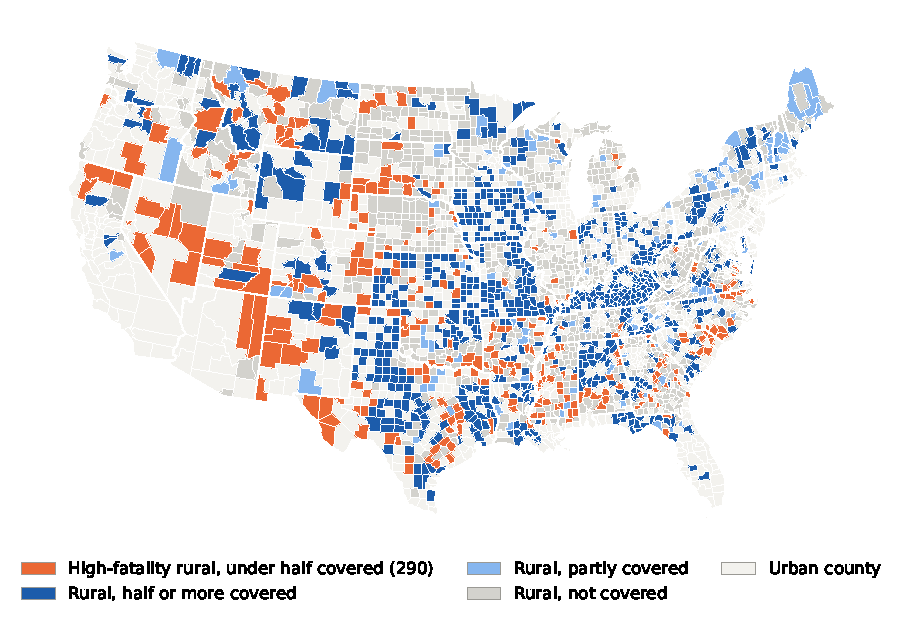
\includegraphics[width=\textwidth]{figures/fig_map.pdf}
\caption{Rural counties by funded SS4A action plan coverage, FY2022--2026, contiguous United States. Orange marks high-fatality rural counties with less than half of residents in a funded plan area (gap counties). Alaska and Hawaii are included in the analysis but not shown.}
\label{fig:map}
\end{figure}

\begin{table}[H]
\centering
\caption{The ten gap counties with the most traffic deaths, 2020--2024. Share is the fraction of 2020 residents inside an SS4A action plan area. Neighbor is a regional body with a funded action plan reaching a bordering county.}
\label{tab:top}
\small
\begin{tabular}{lrrrl}
\toprule
County & Deaths & Death rate & Share & Neighbor \\
\midrule
Robeson County, NC & 293 & 50.1 & 0.00 & Myrtle Beach MPO \\
Navajo County, AZ & 200 & 36.9 & 0.21 & MetroPlan \\
McKinley County, NM & 136 & 38.6 & 0.06 & Mid-Region COG \\
Apache County, AZ & 126 & 38.6 & 0.31 & -- \\
Darlington County, SC & 105 & 33.6 & 0.00 & -- \\
Duplin County, NC & 105 & 42.6 & 0.00 & Wilmington MPO \\
Columbus County, NC & 100 & 39.9 & 0.00 & Myrtle Beach MPO \\
Halifax County, NC & 89 & 37.3 & 0.00 & -- \\
Marshall County, MS & 89 & 52.4 & 0.00 & MidSouth Dev. District \\
Scotland County, NC & 81 & 48.2 & 0.00 & Triangle J COG \\
\bottomrule
\end{tabular}
\end{table}

\subsection{Applications that were not funded}

Only 7 of the 290 gap counties contained an eligible application that DOT did not fund, and in only 3 of them did the application come from the county itself or a place within it; the others were reached through a regional council or a reservation-wide tribal application. For the remaining 283 gap counties the published lists contain no unsuccessful application, and 255 of these were not reached by any SS4A action plan area. Unfunded applications were far more common in urban counties: 27\% of urban counties contained one, compared with 6\% of other rural counties and 3\% of high-fatality rural counties. Among applicants, funding rates did not differ significantly by county group (Table~\ref{tab:apps}). Planning and demonstration applicants were funded at similar rates in urban (81\%), other rural (83\%), and high-fatality rural counties (87\%; $\chi^2_2=1.58$, $p=0.45$), as were implementation applicants ($\chi^2_2=1.41$, $p=0.49$), although few implementation applications came from high-fatality rural counties. Within the limits of the published lists, the gaps reflect counties that did not apply rather than applications that were turned down.

\begin{table}[H]
\centering
\caption{Funded and unfunded SS4A applicants by the county group of the applicant's main county.}
\label{tab:apps}
\small
\begin{tabular}{llrrr}
\toprule
Grant type and years & County group & Funded & Not funded & Funded (\%) \\
\midrule
Implementation, FY2022--FY2024 & Urban & 140 & 320 & 30 \\
 & Other rural & 10 & 31 & 24 \\
 & High-fatality rural & 2 & 2 & 50 \\
\addlinespace
Planning and demonstration, FY2023--FY2024 & Urban & 852 & 205 & 81 \\
 & Other rural & 185 & 38 & 83 \\
 & High-fatality rural & 39 & 6 & 87 \\
\bottomrule
\end{tabular}
\par\smallskip\footnotesize\raggedright Regional applicants are excluded. Each applicant is assigned to the county holding most of its population. Sources: DOT award map layers and Other Applicants lists \citep{usdot2025oa}.
\end{table}

\subsection{Death rates per mile traveled}

Rural counties recorded 1.79 deaths per 100 million vehicle-miles traveled from 2020 to 2024, compared with 1.31 in urban counties. The rural--urban difference is smaller than on the per-resident measure, partly because rural counties carry more travel per resident. Among rural counties with at least five deaths, the two rates were moderately correlated (Spearman $\rho=0.54$). Defining high-fatality rural counties by travel (at least 2.63 deaths per 100 million vehicle-miles) identifies 448 counties, 231 of which are also high-fatality on the per-resident measure. Their coverage (39\%) was again no higher than that of other rural counties (36\%; $\chi^2_1=1.03$, $p=0.31$), and 273 of them (61\%) were gap counties, 152 of which are gaps on both measures. The central finding therefore does not depend on how high fatality is defined.

\subsection{What predicts coverage}

The regression estimates in Table~\ref{tab:reg} show a consistent relationship between coverage, population, and rurality. In the logistic model with regional indicators, a 10 percentage-point increase in the rural population share is associated with a 2.3 percentage-point reduction in the probability of being covered ($p=0.001$). Doubling county population is associated with an increase of about 3.6 percentage points. Fatality rates, poverty, and median household income are not statistically significant predictors in this specification, and the fractional logit analysis of coverage shares yields a similar pattern. Population and rurality also remain the strongest predictors when state fixed effects are included in a linear probability model; the death-rate association is positive but small and only marginally significant ($p=0.05$). Among rural counties considered separately, none of the five measured county characteristics significantly predicts coverage. This suggests that variation in rural coverage is related to factors not captured by these measures. State alone explains 32\% of the variation in rural county coverage.

\begin{table}[H]
\centering
\caption{Models of county action plan coverage. Coefficients with state-clustered standard errors in parentheses. Models 1 and 4: logistic regression of covered status with Census region indicators. Model 2: linear probability model with state fixed effects. Model 3: fractional logit of the coverage share with region indicators. Death rate per 10 deaths per 100{,}000 per year, capped at 200. Significance: $^{*}p<0.05$, $^{**}p<0.01$, $^{***}p<0.001$.}
\label{tab:reg}
\small
\resizebox{\textwidth}{!}{\begin{tabular}{lcccc}
\toprule
 & (1) Logit & (2) LPM, state FE & (3) Fractional logit & (4) Logit, rural only \\
\midrule
Log population & $0.224$ (0.128) & $0.062^{***}$ (0.018) & $0.261^{*}$ (0.129) & $0.170$ (0.190) \\
Rural share (per 10 pp) & $-0.099^{**}$ (0.031) & $-0.018^{***}$ (0.005) & $-0.088^{**}$ (0.030) & $-0.015$ (0.042) \\
Death rate (per 10) & $0.041$ (0.037) & $0.008$ (0.004) & $0.046$ (0.036) & $0.023$ (0.040) \\
Poverty rate (\%) & $-0.009$ (0.023) & $0.001$ (0.004) & $-0.008$ (0.022) & $-0.003$ (0.026) \\
Log median household income & $-0.002$ (0.582) & $0.085$ (0.094) & $0.039$ (0.558) & $0.047$ (0.832) \\
\midrule
Fixed effects & Region & State & Region & Region \\
Counties & 3{,}134 & 3{,}134 & 3{,}134 & 2{,}007 \\
\bottomrule
\end{tabular}}
\end{table}

\subsection{From plans to construction funding}

Although an action plan is intended to provide a route to implementation funding, the progression was much more common in urban counties (Table~\ref{tab:pipe}). Among 536 urban counties covered by plans from the first two rounds, 27\% subsequently had residents within an implementation award area. The corresponding figure was 7\% for the 454 rural counties covered by early plans and 3\% for the 64 high-fatality rural counties in that group. At the individual recipient level, 6.6\% of the 900 early action plan recipients later won implementation grants in their own names. The difference between DOT's rural and urban recipient categories was not statistically significant (7.8\% against 5.0\%; $\chi^2_1=2.25$, $p=0.13$). No regional council, MPO, or Tribal recipient of an early action plan received a later implementation grant under the same recipient name. This is consistent with the structure of regional planning, where the cities and counties responsible for roads generally apply for the implementation grants rather than the regional planning body.

\begin{table}[H]
\centering
\caption{Progression from early action plans (FY2022--2023) to implementation funding (FY2023--2026).}
\label{tab:pipe}
\small
\begin{tabular}{lrr}
\toprule
 & Units & Later implementation (\%) \\
\midrule
\multicolumn{3}{l}{\textit{Counties covered by early plans; implementation award area reaches county residents}} \\
\quad Urban counties & 536 & 27.2 \\
\quad Rural counties & 454 & 6.8 \\
\quad\quad of which high-fatality rural & 64 & 3.1 \\
\multicolumn{3}{l}{\textit{Early action plan recipients; later implementation grant to the same recipient}} \\
\quad All recipients & 900 & 6.6 \\
\quad Cities & 510 & 7.8 \\
\quad Counties & 170 & 10.0 \\
\quad Regional councils and MPOs & 162 & 0.0 \\
\quad Tribes & 27 & 0.0 \\
\bottomrule
\end{tabular}
\end{table}

\subsection{Dollars and deaths}

Allocating SS4A funding to counties according to the population served reveals a substantial difference between the distribution of dollars and deaths. Urban counties received 89\% of program dollars and accounted for 75\% of traffic deaths, whereas high-fatality rural counties received 2.0\% of dollars despite accounting for 6.3\% of deaths (Table~\ref{tab:dol}, Figure~\ref{fig:dol}). Funding per resident was broadly similar across the three county groups, ranging from \$11 to \$17. Measured against traffic deaths, however, urban counties received \$28{,}563 per death, compared with \$7{,}531 in high-fatality rural counties and \$4{,}063 in gap counties. Differences in implementation funding account for most of this disparity. Overall, gap counties recorded 4.1\% of national traffic deaths but were allocated only 0.7\% of SS4A dollars.

\begin{table}[H]
\centering
\caption{SS4A federal dollars allocated to counties by served population, compared with traffic deaths 2020--2024.}
\label{tab:dol}
\small
\resizebox{\textwidth}{!}{\begin{tabular}{lrrrrrr}
\toprule
County group & Deaths (\%) & Dollars (\%) & \$ per resident & \$ per death & Planning \$ per death & Impl.\ \$ per death \\
\midrule
Urban & 74.7 & 88.8 & 15.38 & 28{,}563 & 8{,}554 & 20{,}009 \\
Other rural & 19.1 & 9.3 & 11.08 & 11{,}688 & 4{,}716 & 6{,}972 \\
High-fatality rural & 6.3 & 2.0 & 17.16 & 7{,}531 & 4{,}976 & 2{,}555 \\
Gap counties & 4.1 & 0.7 & 9.27 & 4{,}063 & 2{,}170 & 1{,}894 \\
\bottomrule
\end{tabular}}
\end{table}

\begin{figure}[H]
\centering
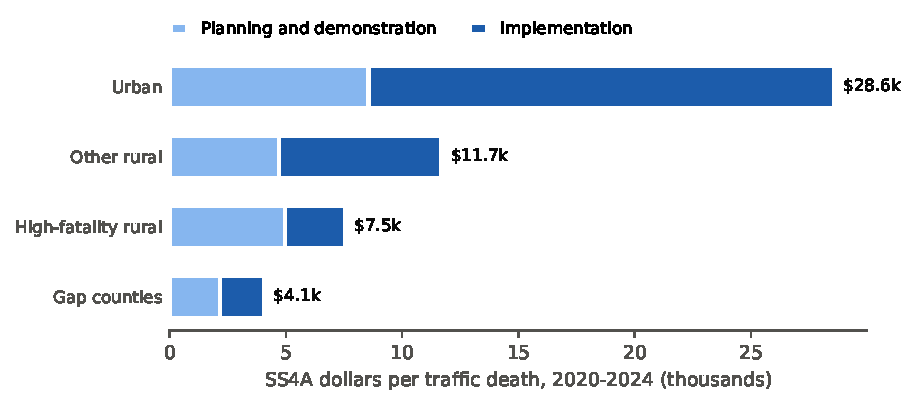
\includegraphics[width=0.72\textwidth]{figures/fig_dollars.pdf}
\caption{SS4A dollars per traffic death (2020--2024) by county group, split into planning and demonstration and implementation awards.}
\label{fig:dol}
\end{figure}

\subsection{The roads on which people die}

The road ownership data point to an additional challenge for gap counties (Table~\ref{tab:roads}). From 2020 to 2024, 73\% of traffic deaths in these counties occurred on state-owned roads, compared with 54\% in urban counties. Only 12\% of deaths in gap counties occurred on roads owned by counties, cities, or towns. Arterials and collectors together accounted for 73\% of their deaths. Local and regional action plans can identify dangerous locations on state highways and provide a basis for working with state departments of transportation. Nevertheless, the roads where most rural deaths occurred were outside the direct control of the local governments eligible for SS4A funding.

\begin{table}[H]
\centering
\caption{Deaths 2020--2024 by road owner and functional class (\% of deaths in each group). Unknown owner and unknown class are not shown.}
\label{tab:roads}
\small
\resizebox{\textwidth}{!}{\begin{tabular}{lrrrrrrr}
\toprule
County group & State & County & City/town & Federal/Tribal & Interstate/fwy & Arterial & Collector/local \\
\midrule
Urban & 53.9 & 12.4 & 20.6 & 0.2 & 19.2 & 54.7 & 25.6 \\
Other rural & 68.5 & 16.9 & 6.6 & 0.2 & 9.7 & 45.4 & 44.3 \\
High-fatality rural & 69.2 & 9.5 & 2.2 & 1.3 & 15.5 & 47.0 & 36.9 \\
Gap counties & 72.7 & 9.9 & 2.3 & 1.6 & 15.8 & 46.0 & 37.6 \\
\bottomrule
\end{tabular}}
\end{table}

\subsection{Spatial clustering and state differences}

Plan coverage also has a clear spatial pattern. Global Moran's $I$ is 0.40 for county coverage shares (permutation $p=0.001$) and 0.15 for the gap indicator ($p=0.001$), indicating geographic clustering in both measures. Local Moran statistics identify 430 counties in low-coverage clusters, meaning that they are surrounded by other counties with low coverage. Of these counties, 83\% are rural, and 27\% of all gap counties lie within these clusters (Figure~\ref{fig:lisa}). Coverage of rural counties differs considerably across states, ranging from 0\% to 100\%, with an interquartile range of 14 to 50\%. In 4 states, no rural county had majority coverage.

Some of this state variation may reflect safety planning that preceded SS4A. In the seven states FHWA previously identified as having established local road safety programs, 21\% of rural counties were covered by SS4A plans, compared with 40\% in other states ($\chi^2_1=48.1$, $p<0.001$). A larger share of their high-fatality rural counties were also gap counties: 76\%, against 63\% elsewhere. Minnesota provides an example: it had funded county road safety plans for all 87 of its counties before SS4A was introduced \citep{mndot2015}. Lower SS4A coverage in these states may therefore indicate reliance on earlier or alternative planning programs rather than a lack of safety planning.

\begin{figure}[H]
\centering
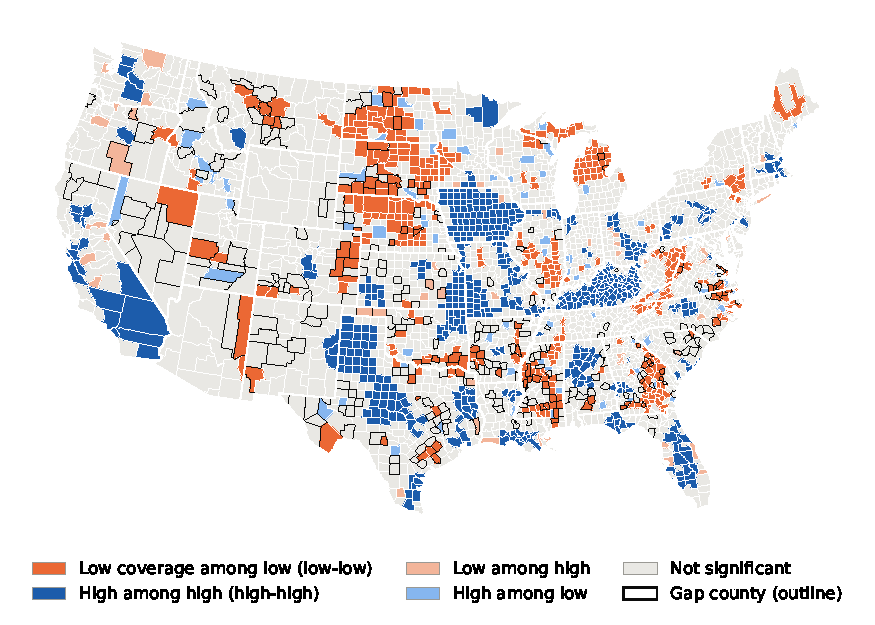
\includegraphics[width=\textwidth]{figures/fig_lisa.pdf}
\caption{Local Moran clusters of the county coverage share ($p<0.05$, 999 permutations, queen contiguity), contiguous United States. Low--low: low coverage surrounded by low coverage. Outlined counties are gap counties.}
\label{fig:lisa}
\end{figure}

\section{Discussion}\label{sec:discussion}

SS4A funded action plans that reached most U.S.\ residents, and DOT's award counts indicate that about half went to communities classified as rural. Yet the county-level coverage measures tell a more uneven story. Rural counties were substantially less likely than urban counties to be reached, and that difference grew over successive rounds. Even within rural America, counties with the highest traffic death rates were not more likely to be covered than other rural counties. Instead, coverage was associated mainly with population and urbanization. Funding was also concentrated in urban counties, where early action plans were more often followed by grants supporting construction. These patterns matter because moving from planning to implementation is a central feature of the program's design.

The application lists add an important qualification. Within the rounds DOT documented, gap counties were almost never turned down; they rarely appear among applicants at all, and rural applicants were funded at rates similar to urban ones. The gaps therefore appear to arise before selection, in whether a county or its regional council applies, rather than in how DOT chose among applications. This points to staff capacity, awareness, and matching funds as the binding constraints, and to outreach and technical assistance rather than changes to scoring as the more promising response.

The program's application process may help explain these differences. Competition for awards requires eligible proposals and local matching funds, advantages more readily available to jurisdictions with planning staff and experience managing grants \citep{smith2025,fast2024}. Rural communities often depend on regional organizations to meet those demands, but action plan awards to regional bodies declined in every round as SS4A increasingly funded implementation. Larger implementation grants bring additional demands, including project design and construction management, that may be difficult for small rural governments to meet. The fact that the measured county characteristics were not significant predictors among rural counties, while state accounted for a large share of their coverage variation, suggests that regional institutions, state arrangements, and local initiative may have mattered more than the characteristics available in the county data.

Road ownership further complicates the picture. Most deaths in gap counties occurred on state highways, where local and regional agencies cannot act independently of state transportation departments. A local safety action plan can still identify hazardous state routes, support coordination, and establish eligibility for supplemental and implementation grants covering measures within local authority. Even so, SS4A's direct influence over the state highways carrying much of the rural fatality burden remains limited. This places the program alongside the state Highway Safety Improvement Program, through which much of the safety investment on those roads is directed.

Not every gap in SS4A coverage indicates an absence of a safety plan. States with established local road safety programs had lower rural SS4A coverage as a group, and some had already financed plans for their counties. Minnesota is a particularly clear example. Implementation awards to Modoc County, California, and McKenzie County, North Dakota, both classified as gap counties here, also indicate that eligible plans can exist without an SS4A planning award. The gap table should therefore be read as a map of where SS4A-funded planning did not reach, not as a complete inventory of counties lacking safety plans. It provides a starting point for checking what planning support is already in place.

\subsection{Implications for policy and practice}

These findings suggest several ways to direct future planning support. The gap table can help regional councils, state transportation departments, and technical assistance providers identify high-fatality rural counties that lack SS4A-funded plan coverage. In 130 gap counties, a regional body already has a funded plan in a bordering county, creating a possible starting point for extending assistance. If SS4A or a successor program receives renewed authorization, reserving some planning funds for high-fatality counties without plans, or offering support outside a competitive process, could help address differences in application capacity \citep{smith2025}. Closer coordination between local plans and state highway safety programs is also important in rural areas, where most deaths occur on roads managed by the state.

\subsection{Limitations}

The findings need to be interpreted in light of several limitations. Coverage identifies action plans funded through SS4A, not all safety plans that may exist. Some counties outside the mapped areas may have plans paid for by state or other sources. An award also does not establish that a plan has been adopted, particularly for plans funded in the last two rounds. The award boundaries come from DOT mapping layers. Although identifiable errors were corrected during reconciliation, an incorrectly located area within the right state might remain undetected, and 55 action plan boundaries may overstate their actual reach. Coverage was calculated using block-group population centers, which means that 64 small award areas containing no such center contributed no covered population. Allocating funds by population served provides an approximation, not a direct measure of where project spending occurred. The fatality measure uses deaths per resident rather than vehicle miles traveled, potentially producing high rates in sparsely populated counties with substantial through traffic. The regressions describe associations and do not include direct measures of government capacity, such as staffing and budgets. The comparison of states with established local road safety programs relies on a list compiled in 2010 and should be understood as illustrative, not causal. Finally, the thresholds used to classify counties as rural, high-fatality, or covered are analytical choices; the released county data allow researchers to examine other definitions. The lists of unfunded applications cover FY2022 to FY2024 only; the FY2022 list includes implementation applications only, and the FY2023 list includes only 7 unfunded planning applications, so a county may have applied in a round for which no list was published. Vehicle-miles traveled from HPMS omit most local-road travel and refer to 2024 only.

\section{Conclusion}\label{sec:conclusion}

Across five years of SS4A awards, funded action plans came to cover most of the U.S.\ population. Coverage nevertheless remained limited in the rural counties with the highest traffic death rates: about two in three still lacked a funded plan reaching most residents. These counties accounted for more of the nation's traffic deaths than of SS4A funding, and most of their deaths occurred on state highways. These gaps also clustered geographically. County population and urbanization were more closely associated with plan coverage than fatality burden, while the transition from planning to construction funding occurred primarily in urban areas. The award-level dataset and county gap table released with this study identify the counties left outside SS4A-funded planning and the regional organizations already holding plans nearby. They can help target technical assistance and future resources toward rural communities facing the highest traffic death rates.

\section*{Data availability}

The award data set with award areas, the county coverage gap table, the regional body table, crosswalks, the unfunded-application crosswalk, county travel measures, the quality report, and all code are available at \url{https://github.com/Emmanuel-Oti-Nani/ss4a-safety-action-plan-coverage} and archived at \href{https://doi.org/10.5281/zenodo.24250593}{doi:10.5281/zenodo.24250593} under CC BY 4.0 (data) and MIT (code) licenses.

\section*{Declarations}

\textbf{Funding.} None. \textbf{Competing interests.} None. \textbf{Ethics.} Analysis of public, de-identified federal data. \textbf{Author contributions.} Emmanuel Oti Nani: conceptualization, methodology, data curation, formal analysis, investigation, writing (original draft, review and editing). Sedinam Annie Barney: conceptualization, methodology, literature review, writing (review and editing). \textbf{Use of AI tools.} Claude (Anthropic) assisted with code, data assembly, and copy-editing; the authors designed and drafted the study, made the analytic decisions, verified the reported figures against the source files, and are responsible for the content.

\begin{thebibliography}{99}
\setlength{\itemsep}{2pt}
\small

\bibitem[Anderson et~al.(2010)]{anderson2010} Anderson, R., Yunk, K., Lovas, D., Scism, M., 2010. Noteworthy Practices: Addressing Safety on Locally-Owned and Maintained Roads. A Domestic Scan. Report FHWA-SA-10-027. Federal Highway Administration, Washington, DC.

\bibitem[Anselin(1995)]{anselin1995} Anselin, L., 1995. Local indicators of spatial association---LISA. Geographical Analysis 27 (2), 93--115. \href{https://doi.org/10.1111/j.1538-4632.1995.tb00338.x}{doi:10.1111/j.1538-4632.1995.tb00338.x}

\bibitem[Beck et~al.(2017)]{beck2017} Beck, L.F., Downs, J., Stevens, M.R., Sauber-Schatz, E.K., 2017. Rural and urban differences in passenger-vehicle-occupant deaths and seat belt use among adults---United States, 2014. MMWR Surveillance Summaries 66 (17), 1--13. \href{https://doi.org/10.15585/mmwr.ss6617a1}{doi:10.15585/mmwr.ss6617a1}

\bibitem[Census Bureau(2022)]{census2022} U.S. Census Bureau, 2022. 2020 Census qualifying urban areas and final criteria clarifications. Federal Register 87, 80114--80154, December 29, 2022.

\bibitem[Census Bureau(2023a)]{censuscb} U.S. Census Bureau, 2023a. 2020 cartographic boundary files: counties, places, and county subdivisions, 1:500{,}000 [data set]. \url{https://www2.census.gov/geo/tiger/GENZ2020/shp/}

\bibitem[Census Bureau(2021)]{censuscenpop} U.S. Census Bureau, 2021. Centers of population for the 2020 Census, block groups [data set]. \url{https://www2.census.gov/geo/docs/reference/cenpop2020/blkgrp/}

\bibitem[Census Bureau(2024)]{saipe2023} U.S. Census Bureau, 2024. Small Area Income and Poverty Estimates, 2023 state and county estimates [data set]. \url{https://www2.census.gov/programs-surveys/saipe/datasets/2023/2023-state-and-county/}

\bibitem[DOT(2026a)]{dotss4a} U.S. Department of Transportation, 2026a. Safe Streets and Roads for All (SS4A) grant program. \url{https://www.transportation.gov/grants/SS4A} (accessed November 10, 2026).

\bibitem[DOT(2026b)]{dotlayers} U.S. Department of Transportation, 2026b. SS4A award map layers, FY2022--FY2026 [data set]. ArcGIS Online. \url{https://services.arcgis.com/xOi1kZaI0eWDREZv/arcgis/rest/services} (accessed November 10, 2026).

\bibitem[DOT(2026c)]{dotlists} U.S. Department of Transportation, 2026c. SS4A full award lists, FY2022--FY2026 [data sets]. \url{https://www.transportation.gov/grants/ss4a/2026-full-award-list} and corresponding pages for earlier years (accessed November 10, 2026).

\bibitem[Fast(2024)]{fast2024} Fast, A., 2024. Safe Streets grants are supposed to save lives. Why are they missing so many deadly roads? USA TODAY, February 2024.

\bibitem[FHWA(2012)]{fhwa2012} Federal Highway Administration, 2012. Developing Safety Plans: A Manual for Local Rural Road Owners. Report FHWA-SA-12-017. Washington, DC.

\bibitem[FHWA(2014)]{fhwa2014} Federal Highway Administration, 2014. Integrating Safety in the Rural Transportation Planning Process. Report FHWA-SA-14-102. Washington, DC.

\bibitem[FHWA(2026)]{fhwa2024hpms} Federal Highway Administration, 2026. Highway Performance Monitoring System, 2024 public release (state HPMS feature services). U.S. Department of Transportation, Washington, DC. \url{https://geo.dot.gov/server/rest/services/Hosted} (accessed November 19, 2026).

\bibitem[FHWA(n.d.)]{fhwass4a} Federal Highway Administration, n.d. Safe Streets and Roads for All (SS4A): Bipartisan Infrastructure Law fact sheet. \url{https://www.fhwa.dot.gov/infrastructure-investment-and-jobs-act/ss4a_fact_sheet.cfm}

\bibitem[Henning-Smith and Kozhimannil(2018)]{henningsmith2018} Henning-Smith, C., Kozhimannil, K.B., 2018. Rural--urban differences in risk factors for motor vehicle fatalities. Health Equity 2 (1), 260--263. \href{https://doi.org/10.1089/heq.2018.0006}{doi:10.1089/heq.2018.0006}

\bibitem[IIJA(2021)]{iija2021} Infrastructure Investment and Jobs Act, 2021. Pub.\ L.\ No.\ 117-58, \S\,24112, 135 Stat.\ 429.

\bibitem[ITF(2016)]{itf2016} International Transport Forum, 2016. Zero Road Deaths and Serious Injuries: Leading a Paradigm Shift to a Safe System. OECD Publishing, Paris. \href{https://doi.org/10.1787/9789282108055-en}{doi:10.1787/9789282108055-en}

\bibitem[MnDOT(2015)]{mndot2015} Minnesota Department of Transportation, 2015. Minnesota Highway Safety Improvement Program 2015 Annual Report. Federal Highway Administration, Washington, DC. \url{https://safety.fhwa.dot.gov/hsip/reports/pdf/2015/mn.pdf}

\bibitem[Moran(1950)]{moran1950} Moran, P.A.P., 1950. Notes on continuous stochastic phenomena. Biometrika 37 (1--2), 17--23. \href{https://doi.org/10.1093/biomet/37.1-2.17}{doi:10.1093/biomet/37.1-2.17}

\bibitem[Nani(2026a)]{nani2026panel} Nani, E.O., 2026a. U.S. Rural Road Fatality County Panel, 2015--2024 (version 1.0.0) [data set and code]. Zenodo. \href{https://doi.org/10.5281/zenodo.23547649}{doi:10.5281/zenodo.23547649}

\bibitem[Nani(2026b)]{nani2026valid} Nani, E.O., 2026b. How rural is rural? Agreement between the FARS rural/urban label and 2020 Census urban areas for U.S.\ traffic deaths, 2015--2024. EarthArXiv preprint. \href{https://doi.org/10.31223/X5RV4C}{doi:10.31223/X5RV4C}

\bibitem[NHTSA(2026)]{nhtsa2026} National Highway Traffic Safety Administration, 2026. Traffic Safety Facts 2024 Data: Rural/Urban Traffic Fatalities. Report DOT HS 813 828. U.S. Department of Transportation, Washington, DC.

\bibitem[Papke and Wooldridge(1996)]{papke1996} Papke, L.E., Wooldridge, J.M., 1996. Econometric methods for fractional response variables with an application to 401(k) plan participation rates. Journal of Applied Econometrics 11 (6), 619--632.

\bibitem[Peek-Asa et~al.(2004)]{peekasa2004} Peek-Asa, C., Zwerling, C., Stallones, L., 2004. Acute traumatic injuries in rural populations. American Journal of Public Health 94 (10), 1689--1693. \href{https://doi.org/10.2105/AJPH.94.10.1689}{doi:10.2105/AJPH.94.10.1689}

\bibitem[Rey and Anselin(2007)]{rey2007} Rey, S.J., Anselin, L., 2007. PySAL: A Python library of spatial analytical methods. Review of Regional Studies 37 (1), 5--27.

\bibitem[Seabold and Perktold(2010)]{seabold2010} Seabold, S., Perktold, J., 2010. Statsmodels: Econometric and statistical modeling with Python. In: Proceedings of the 9th Python in Science Conference, pp.\ 92--96.

\bibitem[Smith et~al.(2025)]{smith2025} Smith, K.K., Goto, E.A., Domingue, S.J., Kalafatis, S.E., Bartley, M.L., Preston, T.L., Hernandez, P.G., 2025. Mapping rural local government capacity for climate resilience projects in the United States. Public Administration Review. \href{https://doi.org/10.1111/puar.70025}{doi:10.1111/puar.70025}

\bibitem[USDOT(2022)]{nrss2022} U.S. Department of Transportation, 2022. National Roadway Safety Strategy. Washington, DC. \url{https://www.transportation.gov/nrss/usdot-national-roadway-safety-strategy}

\bibitem[USDOT(2025)]{usdot2025oa} U.S. Department of Transportation, 2025. SS4A FY22, FY23, and FY24 Other Applicants (eligible applications not selected for funding). Washington, DC. \url{https://www.transportation.gov/grants/ss4a/fy24-other-applicants} (accessed November 19, 2026).

\bibitem[Zwerling et~al.(2005)]{zwerling2005} Zwerling, C., Peek-Asa, C., Whitten, P.S., Choi, S.-W., Sprince, N.L., Jones, M.P., 2005. Fatal motor vehicle crashes in rural and urban areas: decomposing rates into contributing factors. Injury Prevention 11 (1), 24--28. \href{https://doi.org/10.1136/ip.2004.005959}{doi:10.1136/ip.2004.005959}

\end{thebibliography}

\end{document}
